\section{Конструкторская часть}

В данном разделе описан разработанного метод и архитектуры системы, представлены механизмы защиты и примеры их использования для виртуализации функций доверенной среды исполнения.

\subsection{Описание архитектуры системы}\label{sect:arch}

Разработанный метод предполагает использование принципа разделения функциональности на разные компоненты системы. Система спроектирована таким образом, что при атаке или получении доступа к одному из компонентов, её целостность нарушена не будет. Для корректной работы метода, система обязательно должна поддерживать технологию ARM TrustZone и аппаратные механизмы виртуализации ARM. 

Каждой гостевой виртуальной машине сопоставляется виртуальная машина выполняющая роль доверенной среды исполнения, для достижения данной цели используется гипервизор. Каждая виртуальная машина выполняется в обычном мире.

Для обеспечения целостности и проверки последовательности загрузки используется безопасный мир (который является частью ARM TrustZone). В безопасном мире располагаются модули отображения адресов памяти гипервизора и виртуальных машин; модуль перехода и сохранения контекста между виртуальными машинами. Такой подход обеспечивает целостность данных, даже если код гипервизора был скомпрометирован.

Каждая ДСИ использует своё индивидуальное рабочее окружение, в котором хранятся данные. Окружение закреплено за конкретной виртуальной машиной и доступное только когда процессор выполняется в режиме hypervisor, с помощью чего и добивается изоляция. При этом, само окружение не является частью сущности гипервизора.

Для корректного и безопасного взаимодействия вышеописанных компонентов: модулей расположенных в безопасном мире, рабочих окружений и виртуальных машин используется модуль блокировки потока управления, который является частью гипервизора.

На рисунке \ref{fig:full-design} представлена схема разработанной системы.

\begin{figure}[h]
	\centering
	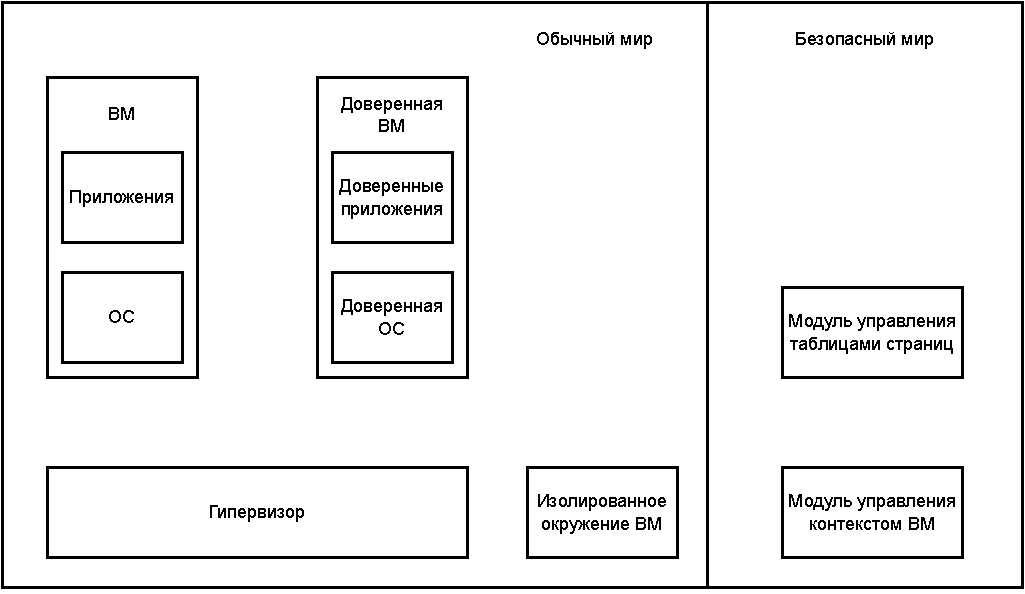
\includegraphics[width=\textwidth]{img/full-design.pdf}
	\caption{Концептуальная схема разработанной системы.}
	\label{fig:full-design}
\end{figure}

\subsection{Механизмы защиты}

Для корректной работы разработанного метода используется модули и окружения, которые были описаны в разделе \ref{sect:arch}. Далее будет дано подробное описание этих механизмов защиты.

\subsubsection{Модуль защищенного отображения памяти}

Модуль отображения памяти отвечает за трансляцию виртуальных адресов в физические в режиме выполнения hypervisor, а так же промежуточных виртуальных в физические для гостевых виртуальных машин. Модуль выполняется в безопасном мире и предоставляет два интерфейса для гипервизора, которые позволяют загрузить и модифицировать таблицу страниц.

Система построена таким образом, что модуль отображения памяти обладает монопольным доступом к загрузке и модификации таблицы страниц. Это достигается с помощью следующих вещей:

\begin{itemize}
	\item [---] Гипервизор не может изменять регистр, в котором хранится указатель на таблицу страниц: все инструкции, позволяющие это сделать, удаляются из его исходного кода. Сами страницы памяти, на которых располагаются таблицы страниц, помечаются как только для чтения для гипервизора.

	\item [---] Страницы памяти, на которых расположен код гипервизора, помечаются как только для чтения. Это позволяет гарантировать что исходный код не может быть изменен во время исполнения.

	\item [---] После запуска системы ни одна страница в адресном пространстве гипервизора не может быть помечена как исполняемая.
\end{itemize}

Таким образом, для внесения изменения в таблицу страниц необходимо использовать интерфейсы предоставляемые модулем отображения памяти, который управляет и реализует различные политики безопасности на каждое такое изменение.

\subsubsection{Модуль блокировки потока управления}

Чтобы принудительно передать управление на определенный код при возникновении какого-либо исключения используется модуль блокировки потока управления, который является частью гипервизора.

В архитектуре ARM, при возникновении исключения, управление передаётся специальному обработчику, адрес которого находится в таблице исключений. Код гипервизора модифицирован таким образом, что он лишён возможности модифицировать регистр содержащий базовый адрес таблицы, а так же её элементы. В обработчики исключений, адреса которых указаны в этой таблице, добавлены специальные инструкции, которые гарантируют перенаправление потока управления к необходимым модулям (например, к модулю переключения контекста).

\subsubsection{Модуль переключения контекста}

Для переключения между контекстами виртуальных машин и гипервизора используется модуль, который выполняется в безопасном мире. Модуль отвечает за переключение между гостевой и доверенной виртуальной машиной и за переключения между виртуальными машинами и гипервизором. Оба типа переключений обрабатываются единообразно, так как в первом случае переключения так же обрабатывает гипервизор.

В архитектуре ARM существует две ситуации, которые могут привести к переключению выполнения из виртуальной машины в гипервизор:

\begin{enumerate}
	\item аппаратное прерывание;
	\item программное прерывание (вызов специальной инструкции процессора) или обработка исключительной ситуации.
\end{enumerate}

В обоих случаях, переключение вызвано исключением, обработка которого будет произведена в данном модуле. Это гарантируется модулем блокировки потока управления.

Гипервизор может переключиться в контекст исполнения виртуальной машины изменив режим привилегий процессора из hypervisor (EL2) в kernel (EL1). Этого можно добиться тремя способами:

\begin{enumerate}
	\item с помощью инструкции eret;
	\item с помощью инструкции movs pc, lr;
	\item явно установить режим привилегий.
\end{enumerate}

Все данные вызовы в исходном коде гипервизора должны быть удалены и заменены на соответствующие вызовы предоставляемые модулем переключения контекста.

\subsubsection{Индивидуальное рабочее окружение}

За каждой доверенной виртуальной машиной закреплено индивидуальное рабочее окружение, выполняемое в режиме работы процессора hypervisor, которое эмулирует функциональность ARM TrustZone. Оно обладает своей таблице страниц, стеком, данными и secure

Каждое окружение удовлетворяет следующим требованиям, которые позволяют его защитить, в случае если гипервизор был скомпрометирован:

\begin{itemize}
	\item [---] Единая точка входа.
	\item [---] Запрещены прерывания. Код должен выполняться от точки входа до точки выхода.
	\item [---] Нет зависимости от данных гипервизора.
	\item [---] Данные окружения не передаются гипервизору.
\end{itemize}

Код каждого рабочего окружения загружается по фиксированному адресу в памяти, который задаётся на стадии компиляции, во время инициализации виртуальной машины. Модули, расположенные в безопасном мире, обладают информацией о метаданных каждого рабочего окружения (адрес точки входа и точки выхода). Сами страницы кода окружения помечаются как только для чтения. Первая и последняя выполняемая инструкция -- это smc. 

Входные данные (получаемые от виртуальной машины), доступны в режиме только для чтения. Для выходных данных выделяются отдельные страницы, так же доступные только для чтения. Чтобы записать в эти страницы какие-либо данные, необходимо сделать запрос к модулю отображения памяти. 

Перед тем как передать управление коду рабочего окружения, страницы его стека настраиваются таким образом, что они доступны для чтения и записи только для ядра процессора, на котором сейчас выполняется его код. Так же, страницы его исходного кода помечаются как доступные для выполнения. Противоположные действия выполняются после исполнения последней инструкции рабочего окружения (smc). За эти действия отвечает модуль отображения памяти, находящийся в безопасном мире.

На рисунке \ref{fig:ciee} представлена схема работы индивидуального рабочего окружения и взаимодействия с другими компонентами системы.

\begin{figure}[h]
	\centering
	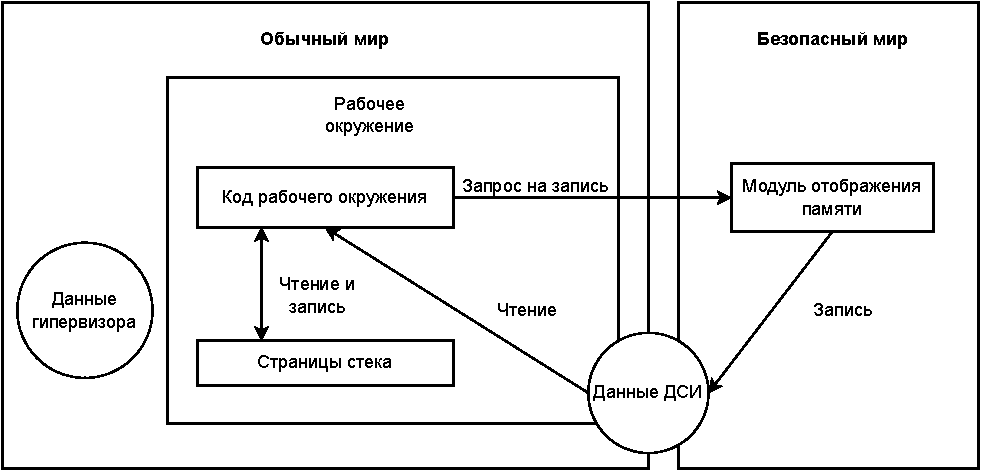
\includegraphics[width=\textwidth]{img/ciee.pdf}
	\caption{Схема работы индивидуального рабочего окружения}
	\label{fig:ciee}
\end{figure}

\subsection{Виртуализация функций ДСИ}

\subsubsection{Доверенная загрузка}

\subsubsection{Состояние ядер процессора}

\subsubsection{Разделение ресурсов системы}

\subsection{Вывод}

\pagebreak
